\nnarticleheader{Random Variables}{Adamya Aggarwal, Haverford '22}

\section*{Random Variables}
In experiments, we are sometimes more interested in some value associated with an event as opposed to the actual event itself. Consider an experiment that flips a coin 5 times. We may not actually care that the order is TTHTH, but we do care about the number of heads that occur (in this case, 2). These values of interest are called random variables.

\begin{definition}
    A discrete random variable $X$ on a sample space $\Omega$ is a function that assigns each sample point $\omega \in \Omega$ a real value $X(\omega)$.
\end{definition}

Note: $\Omega$ is the set of all possible outcomes of an experiment, and $\omega$ is one such outcome.

\vspace{2.5mm}

For a random variable $X$ and a real value $j$, the event $X = j$ is the set of outcomes in $\Omega$ for which $X$ assumes the value $j$. That is, 
\[
X = j \equiv \{\omega \in \Omega | X(\omega) = j \}
\]

\begin{definition}
    An indicator/dummy/binary/Bernoulli variable (there are many names for it) is a random variable that only takes the value 0 or 1.
\end{definition}

\begin{definition}
    The probability mass function (PMF), denoted by $p_{X}$, gives the probability that a random variable $X$ is exactly equal to some value $x$. It can be represented mathematically as follows:
    \[
    p_{X}(x) = \Pr[X = x]
    \]
\end{definition}

Note that 
\[
\sum_{x} p_{X}(x) = \sum_{x} \Pr[X = x] = 1
\]
This is because the events $X = x$ are disjoint and thus partition the sample space $\Omega$. (Going back to the 5 coin flip example, this is logical because for example, there cannot be both 2 and 3 heads in any given sequence.)

\begin{definition}
    Two random variables X and Y are independent if and only if
    \[
    \Pr[X = x \cap Y = y] = \Pr[X = x] \times \Pr[Y = y]
    \]
\end{definition}

Simply put, X and Y are independent if the occurrence of one does not affect the probability of occurrence of the other.

\section*{Expectation}

\begin{definition}
    The expected value of a random variable $X$ is a weighted average of the possible values that X can take. The expectation is what you would expect the outcome of an experiment to be on average.
    \[
    \E[X] = \sum_{x} x p_{X}(x) = \sum_{x} x \Pr[X = x]
    \]
\end{definition}
Note: The expected value of an indicator variable $X_{i}$ is just $\Pr[X_{i} = 1]$.

\vspace{5mm}

\textbf{Example 1:}
In the running example of 5 coin flips, find the expectation of the number of heads.

\vspace{2.5mm}

\textbf{Solution:}
\begin{align*}
\begin{split}
    \E[X] ={}& 0 \times \Pr[X = 0] + 1 \times \Pr[X = 1] + 2 \times \Pr[X = 2] + 3 \times \Pr[X = 3]\\
    & + 4 \times \Pr[X = 4] + 5 \times \Pr[X = 5]
\end{split}\\
    ={}& 0 \times \frac{1}{32} + 1 \times \frac{5}{32} + 2 \times \frac{10}{32} + 3 \times \frac{10}{32} + 4 \times \frac{5}{32} + 5 \times \frac{1}{32} \\
    ={}& 0 + \frac{5}{32} + \frac{20}{32} + \frac{30}{32} + \frac{20}{32} + \frac{5}{32} \\
    ={}& \frac{80}{32} \\
    ={}& 2.5
\end{align*}

Thus, the expected value for the number of heads in any given 5 flips is 2.5. Note that the expectation of a random variable does not necessarily have to be a valid value of the random variable (i.e. there can never actually be 2.5 heads). Think of it this way: if we were to run this experiment an infinite number of times, the average number of heads for all of those experiments would tend toward 2.5.

\vspace{5mm}

\textbf{Example 2:}
If you rolled two dice, in expectation, what is the sum?

\vspace{2.5mm}

\textbf{Solution:} \\
Let S be a random variable that denotes the sum of the roll of the 2 dice.

$$
\Pr[S = s] = 
\begin{cases}
\frac{1}{36} & \text{if $s$ = 2 or 12}\\
\frac{2}{36} & \text{if $s$ = 3 or 11}\\
\frac{3}{36} & \text{if $s$ = 4 or 10}\\
\frac{4}{36} & \text{if $s$ = 5 or 9}\\
\frac{5}{36} & \text{if $s$ = 6 or 8}\\
\frac{6}{36} & \text{if $s$ = 7}\\
\end{cases}
$$

To find the expectation, we can do the following calculations:
\begin{align*}
    \E[X] ={}& \sum_{x=2}^{12} x \Pr[X = x] \\
    \begin{split}
        ={}& (2 + 12) \times \frac{1}{36} + (3 + 11) \times \frac{2}{36} + (4 + 10) \times \frac{3}{36} + (5 + 9) \times \frac{4}{36} \\
        & + (6 + 8) \times \frac{5}{36} + (7) \times \frac{6}{36}
    \end{split} \\
    ={}& 7
\end{align*}

The expected value for the sum of the two dice is 7.

\subsection*{Linearity of Expectation}
Linearity of expectation is the property that the expected value of the sum of random variables is equal to the sum of their individual expected values, regardless of whether they are independent.
\begin{theorem}
    If $X = X_{1} + X_{2} + \ldots + X_{n}, then \E[X] = \E[X_{1}] + \E[X_{2}] + \ldots + \E[X_{n}]$. That is,
    \[
    \E[\sum_{i=1}^{n} X_{i}] = \sum_{i=1}^{n} E[X_{i}]
    \]
\end{theorem}
From linearity of expectation, we can further deduce that E[cX] = cE[X].

\vspace{5mm}

\textbf{Example 3:}
Use linearity of expectation to find the expected sum of 2 dice.

\vspace{2.5mm}

\textbf{Solution:} \\
We still want to find $\E[X]$, but there is another way to arrive at the solution. Let $X_{1}$ and $X_{2}$ be random variables denoting the results of the first and second rolls, respectively. Realize that because $X = X_{1} + X_{2}$,
    $$
    \E[X] = \E[X_{1} + X_{2}]
    $$
    
Using linearity of expectation, we get
    \begin{align*}
        \E[X] &= \E[X_{1}] + \E[X_{2}] \\
        &= \frac{1}{6}(1 + 2 + 3 + 4 + 5 + 6) + \frac{1}{6} (1 + 2 + 3 + 4 + 5 + 6) \\
        &= 7
    \end{align*}
    
\subsection*{The Hat Check Problem}
Suppose n people check in their hats at a hat check. The hats are returned randomly. In expectation, what is the number of people that get their own hat back?

\vspace{2.5mm}

\textbf{Solution:} \\
Let X be a random variable denoting the number of people who get their own hat back. Remember,
    $$
    \E[X] = \sum_{x=0}^{n}x\Pr[X = x]
    $$
But how can we calculate the probability of $x$ people getting their hats back? Let’s use indicator variables to make the problem more manageable. Let $X_{i}$ be an indicator variable that equals 1 if the $i^{\text{th}}$ person gets their hat back and equals 0 otherwise. Then,
    \begin{align*}
        X &= \sum_{i=1}^{n}X_{i} \\
        \E[X] &= \E[\sum_{i=1}^{n}X_{i}]
    \end{align*}
By linearity of expectation,
    $$
    \E[X] = \sum_{i=1}^{n}\E[X_{i}]
    $$
Because $X_{i}$ can only equal 0 or 1, we can rewrite this as
    \begin{align*}
        \E[X] &= \sum_{i=1}^{n}(0 \times \Pr[X_{i} = 0] + 1 \times \Pr[X_{i} = 1]) \\
        &= \sum_{i=1}^{n}\Pr[X_{i} = 1]
    \end{align*}
Notice that $X_{i}$ and $X_{j}$ are not independent because the probability that someone gets his hat back can change depending on if someone earlier already got his back. Say we know that $X_{1}$ got his hat back. Then the probability that $X_{2}$ gets his hat back becomes $\frac{1}{n-1}$.

But independence actually doesn’t matter for linearity. What we need is the unconditional probability that the $i^{\text{th}}$ person gets the right hat, ignoring whether the first guest got the right hat or not. Since there are n hats and all of them are equally likely to be the one that that guest gets, the probability is $\frac{1}{n}$.
    \begin{align*}
        \E[X] &= \sum_{i=1}^{n}\frac{1}{n} \\
        &= n(\frac{1}{n}) \\
        &= 1
    \end{align*}
Thus, we can expect that of $n$ people, 1 person will get their correct hat if they are distributed randomly.

\subsection*{Balls and Bins}
Suppose you throw $n$ balls at $n$ bins, and each ball is equally likely to land in each of the $n$ bins (assume you’ll always make it into one of the bins). What is the expected number of empty bins?

\vspace{2.5mm}

\textbf{Solution:} \\
Let $X$ be a random variable denoting the number of empty bins. Let $X_{i}$ be an indicator variable that is 1 if bin $i$ is empty and 0 otherwise.
    \begin{align*}
        X &= \sum_{i=1}^{n}X_{i} \\
        \E[X] &= \E[\sum_{i=1}^{n}X_{i}] \\
        \E[X] &= \sum_{i=1}^{n}\E[X_{i}] \\
        &= \sum_{i=1}^{n}\Pr[X_{i} = 1]
    \end{align*}
$\Pr[X_{i} = 1] = (1-\frac{1}{n})^{n}$, so
    $$
    \E[X] = \sum_{i=1}^{n}(1-\frac{1}{n})^{n}
    $$
$\lim\limits_{n \to \infty}(1-\frac{1}{n})^{n} = \frac{1}{e}$, so for large enough values of $n$, we have
    $$
    \E[X] \approx \frac{n}{e}
    $$

\section*{Variance}
What if we want to find how much a random variable $X$ deviates from its mean? Intuitively, we would be looking for $\E[X - \E[X]]$. In words, that gives the expected value of the difference between the value of the random variable and the expected value of that variable. Using linearity of expectation, let’s simplify:
    \begin{align*}
        \E[X - \E[X]] &= \E[X] - \E[\E[X]] \\
        &= \E[X] - \E[X] \\
        &= 0
    \end{align*}
Notice that because $\E[X]$ is a constant, $\E[\E[X]]$ is just $\E[X]$. The above result obviously does not help us; we don’t want the positive and negative deviations to cancel each other out because it would tell us that on average, we are never wrong. And this would happen regardless of what the random variable denotes. This suggests we should take the absolute value of $X - \E[X]$. But we actually square it (I’ll explain in brief why shortly), which leads to the definition of variance.

\begin{definition}
    The variance of random variable X is given by
    $$
    \Var[X] = \E[(X - \E[X])^{2}]
    $$
\end{definition}
You might be wondering (rightfully so) why we square instead of taking the absolute value. There are a couple of reasons. I won’t go into too much depth here, but the short answer is \textbf{squaring makes the algebra much easier to work with} than the absolute method. Of course, both squaring and taking the absolute value give a positive value, but squaring puts larger emphasis on outliers (which can be useful) and is continuously differentiable (as opposed to the absolute value function).

\vspace{2.5mm}

Note: The standard deviation of a random variable $X$ is defined as
$$
\sigma[X] = \sqrt{\Var[X]}
$$
This essentially undoes the squaring in variance, and it’s relatively easy to switch from one to the other in calculations.

\vspace{2.5mm}

Here is a simplification of the variance definition using linearity of expectation.
    \begin{align*}
    \E[(X - \E[X])^{2}] &= \E[X^{2} - 2X\E[X] + \E[X]^{2}] \\
    &= \E[X^{2}] - 2\E[XE[X]] + \E[\E[X]^{2}] \\
    &= \E[X^{2}] - 2\E[X]^{2} + \E[X]^{2} \\
    &= \E[X^{2}] - \E[X]^{2}
    \end{align*}

\textbf{Example 4:}
If X is a random variable denoting the sum of two dice, what is Var[X]?

\vspace{2.5mm}

\textbf{Solution:} \\
We know our answer lies in the formula $\E[X^{2}] - \E[X]^{2}$. We have already calculated $\E[X]$ to be 7, so $\E[X]^{2}$ is simply 49.
Now we must find $\E[X^{2}]$

\begin{align*}
    \begin{split}
        \E[X^{2}] ={}& (2^{2} + 12^{2}) \times \frac{1}{36} + (3^{2} + 11^{2}) \times \frac{2}{36} + (4^{2} + 10^{2}) \times \frac{3}{36} + (5^{2} + 9^{2}) \times \frac{4}{36} \\
        & + (6^{2} + 8^{2}) \times \frac{5}{36} + (7^{2}) \times \frac{6}{36}
    \end{split} \\
    ={}& 54.83
\end{align*}

Thus, we have
\begin{align*}
    \Var[X] &= \E[X^{2}] - \E[X]^{2} \\
    &= 54.83 - 49 \\
    &= 5.83
\end{align*}

\subsection*{Variance in the Hat Check Problem}
\textbf{Solution:}\\
We have already calculated $\E[X]$ to be 1, so $\E[X]^{2}$ is just 1. Now we must find $\E[X^{2}]$. This requires a little more work. Remember that
    $$
    X = X_{1} + X_{2} + \ldots + X_{n}
    $$
Squaring both sides, we get
    $$
    X^{2} = \sum_{i}X_{i}^{2} + \sum_{i,j}X_{i}X_{j}
    $$
    
This is because when we multiply $X = X_{1} + X_{2} + \ldots + X_{n}$ by itself and expand the product, we get many different cross terms, some of which will be of the form $X_{i}^{2}$ and others will be of the form $(X_{i})(X_{j})$, where $i \neq j$. $X^{2} = \sum\limits_{i}X_{i}^{2} + \sum\limits_{i,j}X_{i}X_{j}$ just represents the sum of all of those products.

\vspace{2.5mm}

We need to find $\E[X^{2}]$, so using linearity of expectation,
    $$
    \E[X^{2}] = \sum_{i}\E[X_{i}^{2}] + \sum_{i,j}\E[X_{i}X_{j}]
    $$

Let’s split the right-hand side up even further and first find $\E[X_{i}^{2}]$. Remember, $\E[X_{i}]$ can only equal 0 or 1, so
    \begin{align*}
        \E[X_{i}^{2}] &= 0^{2} \times \Pr[X = 0] + 1^{2} \times \Pr[X = 1] \\
        &= \Pr[X = 1] \\
        &= \frac{1}{n}
    \end{align*}
    
Now let's find $\E[X_{i}X_{j}]$. Because $X_{i}$ and $X_{j}$ are both indicator random variables, $X_{i}X_{j}$ can only take the values 0 or 1, meaning it is also an indicator variable. Thus, 
    $$
    \E[X_{i}X_{j}] = \Pr[X_{i}X_{j} = 1]
    $$

For $X_{i}X_{j}$ to equal 1, both $X_{i}$ and $X_{j}$ must equal one, so we can rewrite this as
    $$
    \E[X_{i}X_{j}] = \Pr[X_{i} = 1 \cap X_{j} = 1]
    $$
    
Remember that the events $X_{i}$ are not independent. So to calculate what’s above, we must use conditional probability. That is,
    \begin{align*}
        \E[X_{i}X_{j}] &= \Pr[X_{i} = 1] \times \Pr[X_{j} = 1|X_{i} = 1] \\
        &= (\frac{1}{n})(\frac{1}{n-1})
    \end{align*}
    
\vspace{1.5mm}
    
Going back to the equation $X^{2} = \sum\limits_{i}X_{i}^{2} + \sum\limits_{i,j}X_{i}X_{j}$, realize that the sum $\sum\limits_{i}X_{i}^{2}$ has $n$ terms in it. Furthermore, the sum $\sum\limits_{i,j}X_{i}X_{j}$ must have $n^{2}-n$ terms (because $X^{2}$ must have a total of $n^{2}$ terms in it). Putting this all together, we have
    \begin{align*}
        \E[X^{2}] &= (n)(\frac{1}{n}) + (n^{2}-n)(\frac{1}{n})(\frac{1}{n-1}) \\
        &= 2
    \end{align*}
    
Now we can plug into the variance formula and get
\begin{align*}
    \Var[X] &= \E[X^{2}] - \E[X]^{2} \\
    &= 2 - 1 \\
    &= 1
\end{align*}

\vspace{1cm}

\renewcommand{\thefigure}{1}
\begin{figure}[htp]
    \centering
    \begin{minipage}{10.5cm}
    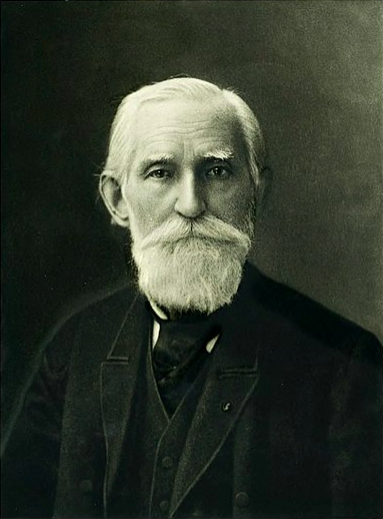
\includegraphics[width=10.5cm]{aggarwal_image1}
    \caption{Pafnuty Chebyshev (1821-1894) was a Russian Mathematician. He is widely acknowledged as the first person to think in terms of random variables. }
    \label{fig:1}
    \end{minipage}
\end{figure}
